% Copyright (c) 2026 Islam Ibrahim. All rights reserved.

\documentclass[tikz,border=8pt]{standalone}
\usepackage[T1]{fontenc}
\usepackage{lmodern}
\usepackage{amsmath}
\usepackage{tikz}
\usetikzlibrary{arrows.meta,decorations.pathmorphing}
\begin{document}
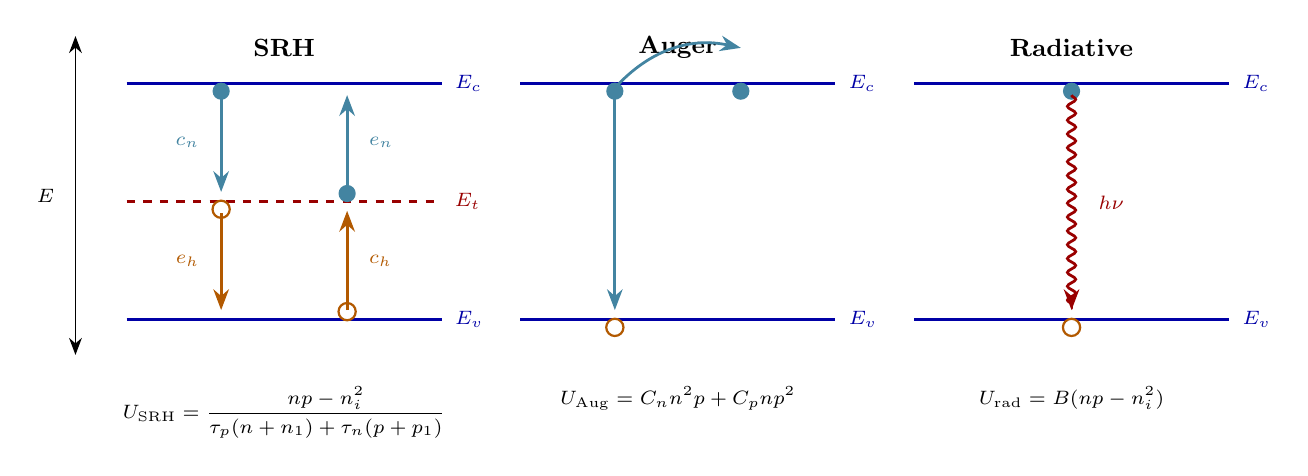
\begin{tikzpicture}[font=\small\rmfamily,>=Stealth,
  band/.style={line width=1.1pt,blue!65!black},
  arr/.style={line width=1.0pt,->},
  lbl/.style={font=\scriptsize\rmfamily},
  ec/.style={circle,fill=cyan!60!black,inner sep=2.2pt},
  hv/.style={circle,draw=orange!70!black,fill=white,inner sep=2.2pt,line width=0.8pt},
  pnl/.style={font=\small\bfseries\rmfamily},
]

%% Layout parameters
\def\bW{4.0}      % band width
\def\sep{5.0}     % panel separation
%% Energy levels
\def\Ec{3.0}
\def\Ev{0.0}
\def\Et{1.5}
%% Pre-computed midpoints
\pgfmathsetmacro{\EcEt}{(\Ec+\Et)/2}
\pgfmathsetmacro{\EtEv}{(\Et+\Ev)/2}

%% ---- Energy axis ----
\draw[<->,line width=0.7pt] (-0.65,-0.45)--(-0.65,3.6)
  node[midway,left=4pt,lbl]{$E$};

%% ================================================================
%%  SRH  (Shockley--Read--Hall)
%% ================================================================
\node[pnl] at (\bW/2,\Ec+0.45) {SRH};

\draw[band] (0,\Ec)--(\bW,\Ec)
  node[right=1pt,lbl,blue!65!black]{$E_c$};
\draw[band] (0,\Ev)--(\bW,\Ev)
  node[right=1pt,lbl,blue!65!black]{$E_v$};
\draw[line width=0.9pt,red!60!black,dashed] (0,\Et)--(\bW,\Et)
  node[right=1pt,lbl,red!60!black]{$E_t$};

\node[ec] at (1.2,\Ec-0.1) {};
\draw[arr,cyan!60!black] (1.2,\Ec-0.15)--(1.2,\Et+0.12);
\node[lbl,cyan!60!black,left=3pt] at (1.15,\EcEt) {$c_n$};

\node[hv] at (1.2,\Et-0.1) {};
\draw[arr,orange!70!black] (1.2,\Et-0.15)--(1.2,0.12);
\node[lbl,orange!70!black,left=3pt] at (1.15,\EtEv) {$e_h$};

\node[ec] at (2.8,\Et+0.1) {};
\draw[arr,cyan!60!black] (2.8,\Et+0.15)--(2.8,\Ec-0.15);
\node[lbl,cyan!60!black,right=3pt] at (2.85,\EcEt) {$e_n$};

\node[hv] at (2.8,\Ev+0.1) {};
\draw[arr,orange!70!black] (2.8,0.12)--(2.8,\Et-0.12);
\node[lbl,orange!70!black,right=3pt] at (2.85,\EtEv) {$c_h$};

\node[lbl,align=center,below=18pt] at (\bW/2,-0.1)
  {$U_\mathrm{SRH}=\dfrac{np-n_i^{2}}{\tau_p(n+n_1)+\tau_n(p+p_1)}$};

%% ================================================================
%%  Auger
%% ================================================================
\node[pnl] at (\sep+\bW/2,\Ec+0.45) {Auger};

\draw[band] (\sep,\Ec)--(\sep+\bW,\Ec)
  node[right=1pt,lbl,blue!65!black]{$E_c$};
\draw[band] (\sep,\Ev)--(\sep+\bW,\Ev)
  node[right=1pt,lbl,blue!65!black]{$E_v$};

%% eeh process — positions relative to sep
\pgfmathsetmacro{\AugA}{\sep+1.2}
\pgfmathsetmacro{\AugB}{\sep+2.8}
\node[ec] at (\AugA,\Ec-0.1) {};
\node[ec] at (\AugB,\Ec-0.1) {};
\node[hv] at (\AugA,-0.10) {};

%% recombination
\draw[arr,cyan!60!black] (\AugA,\Ec-0.15)--(\AugA,0.12);

%% energy transfer to second electron
\draw[arr,cyan!60!black,bend left=30] (\AugA,\Ec-0.06) to (\AugB,\Ec+0.45);

\node[lbl,align=center,below=18pt] at (\sep+\bW/2,-0.1)
  {$U_\mathrm{Aug}=C_n n^{2}p + C_p n p^{2}$};

%% ================================================================
%%  Radiative
%% ================================================================
\node[pnl] at (2*\sep+\bW/2,\Ec+0.45) {Radiative};

\draw[band] (2*\sep,\Ec)--(2*\sep+\bW,\Ec)
  node[right=1pt,lbl,blue!65!black]{$E_c$};
\draw[band] (2*\sep,\Ev)--(2*\sep+\bW,\Ev)
  node[right=1pt,lbl,blue!65!black]{$E_v$};

\pgfmathsetmacro{\RadX}{2*\sep+\bW/2}
\node[ec] at (\RadX,\Ec-0.1) {};
\node[hv] at (\RadX,-0.10) {};

\draw[arr,red!60!black,
  decorate,decoration={snake,amplitude=1.5pt,segment length=5pt}]
  (\RadX,\Ec-0.15)--(\RadX,0.12)
  node[midway,right=6pt,lbl,red!60!black]{$h\nu$};

\node[lbl,align=center,below=18pt] at (2*\sep+\bW/2,-0.1)
  {$U_\mathrm{rad}=B(np-n_i^{2})$};

\end{tikzpicture}
\end{document}
